\documentclass[article,12pt,oneside,a4paper,brazil]{abntex2}

\usepackage[alf]{abntex2cite}
\usepackage{graphicx} % Required for inserting images
\usepackage[utf8]{inputenc}
\usepackage[brazil]{babel}
\usepackage[outline]{contour} % glow around text
\usepackage{lipsum}
\usepackage{amsmath} % For align environment
\usepackage{cancel}
\usepackage{blindtext}
\usepackage{tikz, tkz-base, tkz-fct}
\usepackage{pgfplots}
\usepackage{indentfirst}
\usepackage{multirow}
\usepackage{physics}
\usepackage[T1]{fontenc}    % para suporte a caracteres acentuados
\usepackage{indentfirst}
\usepackage{float}
\usepackage{amsfonts}

\usetikzlibrary{angles,quotes} % for pic
\contourlength{1.2pt}

% Estou colocando 2 de espaço por cada pergunta

% Personalizando as coisas do latex
\usepackage[left=2.5cm,top=2.5cm,right=2.5cm,bottom=2.5cm]{geometry}

\begin{document}
	\section*{7.14 Interpretação de $\frac{dy}{dx}$ como um quociente diferencial}
	
	\subsection*{12.1.1 Teorema: }
	
	\begin{flushleft}	
		
	\end{flushleft}
	
	\subsection*{12.1.2 Notas de Aulas}
	
	\begin{flushleft}
		Agora o $\dfrac{dy}{dx}$ vai ser como um quociente entre dois crescimentos. Sabemos que $f'(x)"$ é o quociente do ângulo da reta $T$, no ponto $P(x, f(x))$. Exemplo
		
		\begin{equation*}
			\dfrac{dy}{dx} = f'(x) = \tan{x}
		\end{equation*}
	
		Podemos isolar apenas o $dy$, deixando a equação da seguinte forma:
		
		\begin{equation*}
			dy = f'(x) \cdot dx
		\end{equation*}
		
		\begin{center}
			\begin{figure}[H]
				\centering
				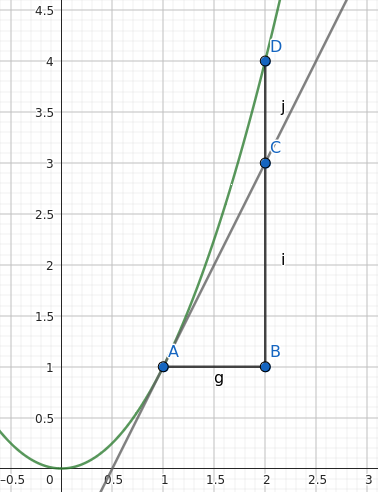
\includegraphics[width=0.4\textwidth, height=5cm]{imagens/GeoGebra.png}
				\caption{Software GeoGebra}
				\label{fig:geogebra}
			\end{figure}
		\end{center}
	
		Observe que há umas letras em minúsculas ao lado de retas pretas no gráfico. A reta $i$ representa a diferenciável $dy$ e a reta $j$ representa a diferencial de $\Delta{y} - dy$.
		
		Além disso, observe que $\Delta{y} = f(x + dx) - f(x)$. Isso é o crescimento que ocorre em $x$ até o $x + dx$. O acrecimo de $\Delta{y}$ pode ser enxergado como um valor aproximado; Evidentemente um erro "$\Delta{y} - dy$".
	\end{flushleft}
	
	\subsection*{12.1.3 Exercícios: }
	\begin{flushleft}	
		\textbf{1.} Cálcule a diferencial.
		
		\textbf{a) } $y = x^3 \Rightarrow dy = 3x^2 \cdot \,dx$ \\[1em]
		
		\textbf{b) } $y = x^2 -2x \Rightarrow dy = \left( 2x - 2 \right) \cdot \,dx$ \\[1em]
		
		\textbf{c) } $y = \frac{x}{x + 1} \Rightarrow dy = \frac{1}{(x + 1)^2} \cdot \,dx$ ,  $\forall x \in \mathbb{R} \setminus \{ -1 \}$ \\[1em]
		
		\textbf{d) } $y = \sqrt[3]{x} \Rightarrow  dy = \frac{1}{3 \cdot \sqrt[3]{x^2}} \cdot dx$ \\[1em]
		
		\textbf{1.} Seja $A = l^2$, $l > 0$.
		
		\textbf{a) } Calcule a diferencial.
		
		\textbf{b) } Interprete geometricamente o erro que se comete na proximação de $\Delta{A}$ por $dA$. (Olhe para $A = l^2$ como a fórmula para o cálculo da área do quadrado de lado $l$).
		
				
	\end{flushleft}
	
	
	
	
\end{document}